\documentclass[10pt]{beamer}
\usetheme{metropolis}
\usepackage{tikz}
\usetikzlibrary{fit,positioning}
\usepackage{attrib}
\usepackage{rotating}
\usepackage{biblatex}
\usepackage{subcaption}
\addbibresource{../bib.bib}

\setbeamerfont{footnote}{size=\tiny}

\usepackage{amsmath}
\DeclareMathOperator*{\argmax}{arg\,max}

\setsansfont{Noto Sans}
\setmonofont{Droid Sans Mono}

\title{Modeling MOOC Student Behavior With Two-Layer Hidden Markov Models}
\author{Chase Geigle and ChengXiang Zhai}
\institute{Department of Computer Science, University of Illinois at
Urbana-Champaign}
\date{2017-06-25}

\begin{document}

\maketitle

\section{Motivation}

\begin{frame}
  \begin{center}
      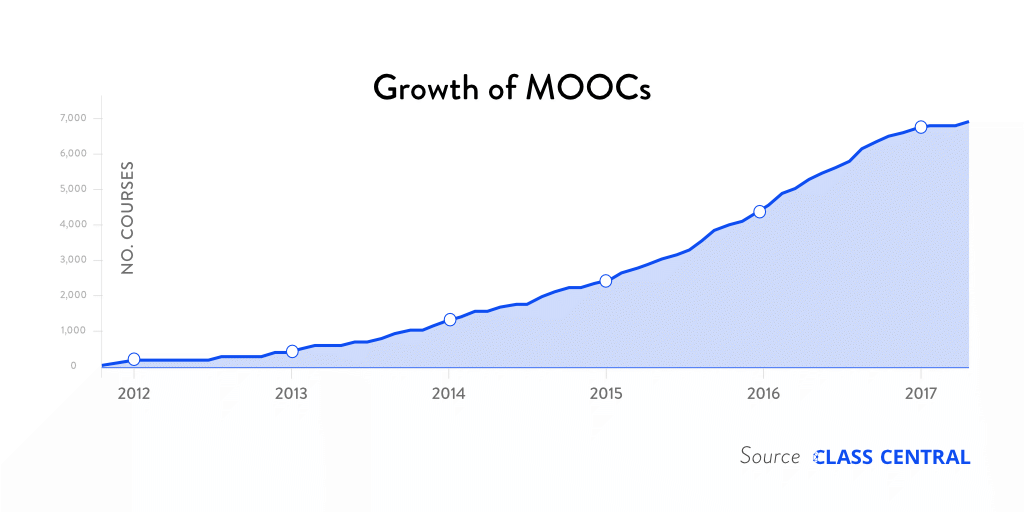
\includegraphics[width=\textwidth]{figures/Growth-of-MOOCs.png}

      \small{\url{https://www.class-central.com/report/moocs-stats-and-trends-2016/}}
  \end{center}
\end{frame}

\begin{frame}{The Back of My Envelope}
  Data looks like:
  \begin{center}
    view lecture \rightarrow\, quiz \rightarrow\, forum \rightarrow\,
    \ldots\, \rightarrow\, view lecture \rightarrow\, quiz \rightarrow\,
    quiz \rightarrow\, forum \rightarrow\, \ldots
  \end{center}

  If every course looked like Cheng's\ldots
  \begin{center}
      \[
        \sim 7,000\text{ courses } \times \frac{\sim 85,000\text{ browsing
        sessions }}{\text{ course }} \times \frac{\sim 7\text{
        actions }}{\text{ browsing session }}
      \]
      \Large
      \begin{align*}
        \approx &\text{ } \mathbf{4.2} \text{ \textbf{billion} actions }
        \\
        &\text{ across } \mathbf{595} \text{ \textbf{million} sessions }
      \end{align*}
  \end{center}
\end{frame}

\begin{frame}{Where we come in\ldots}
    We need \textbf{\alert{concise}} and \textbf{\alert{digestible}}
    summaries of these logs in order to understand them!
    \\[\baselineskip]
    This paper contributes the following:
    \begin{enumerate}
      \item A suggestion for a \textbf{behavior pattern representation} to
       understand patterns and \textbf{transitions between them}, and
       \\[0.5\baselineskip]
      \item A model that can efficiently and \textbf{automatically} capture
       this kind of representation in an \textbf{unsupervised} way
    \end{enumerate}
\end{frame}

\section{Example}

\begin{frame}{Our Behavior Representation}
  Visualize behavior patterns with \textbf{labeled directed graphs} where
  \begin{itemize}
      \item \textbf{node size} is proportional to the \textbf{probability
          of being at that node} at any given time,
          \\[\baselineskip]
      \item a \textbf{directed edge} represents a \textbf{transition from one behavior to
          another}, and
          \\[\baselineskip]
      \item the \textbf{thickness of an edge} is proportional to the
          \textbf{probability of taking that edge} to leave the source node.
  \end{itemize}
\end{frame}

\begin{frame}{(Theoretical Example) Behavior Pattern 0}
  \centering
  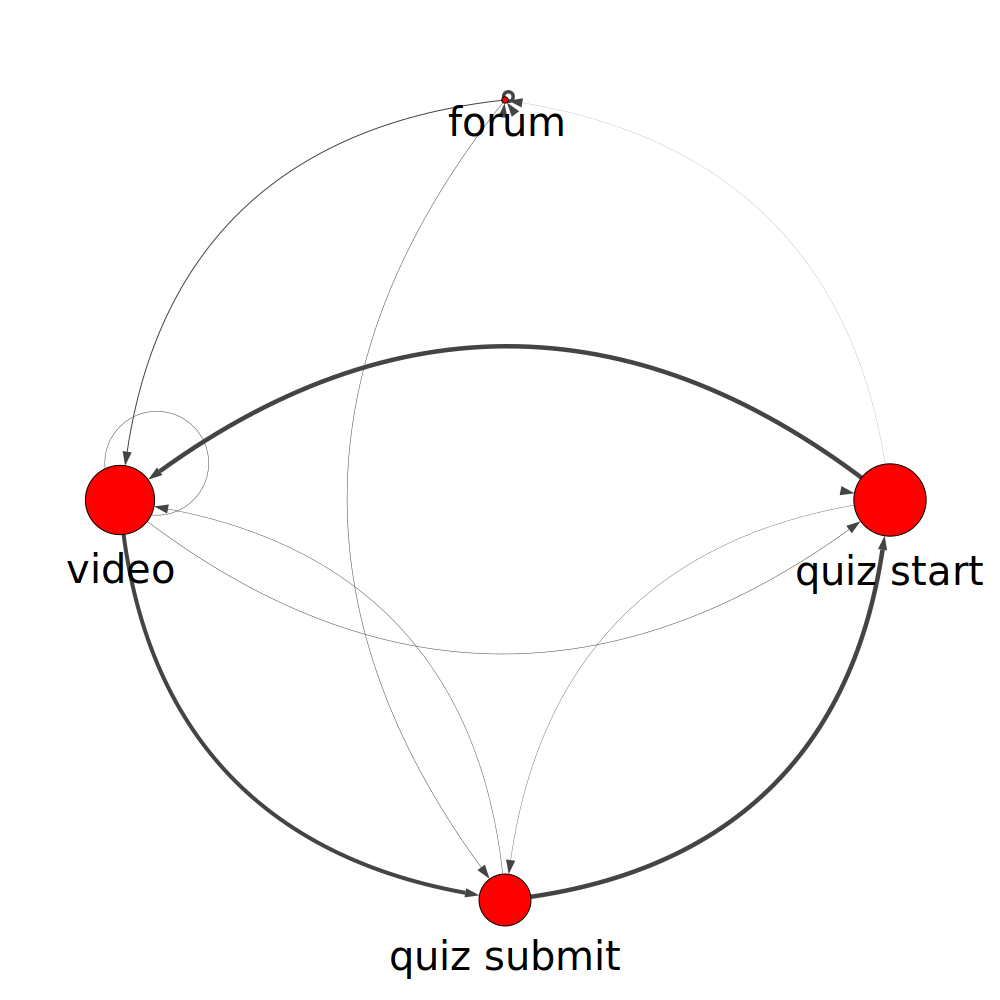
\includegraphics[width=0.7\textwidth]{../figures/example/state0.png}
\end{frame}

\begin{frame}{(Theoretical Example) Behavior Pattern 1}
  \centering
  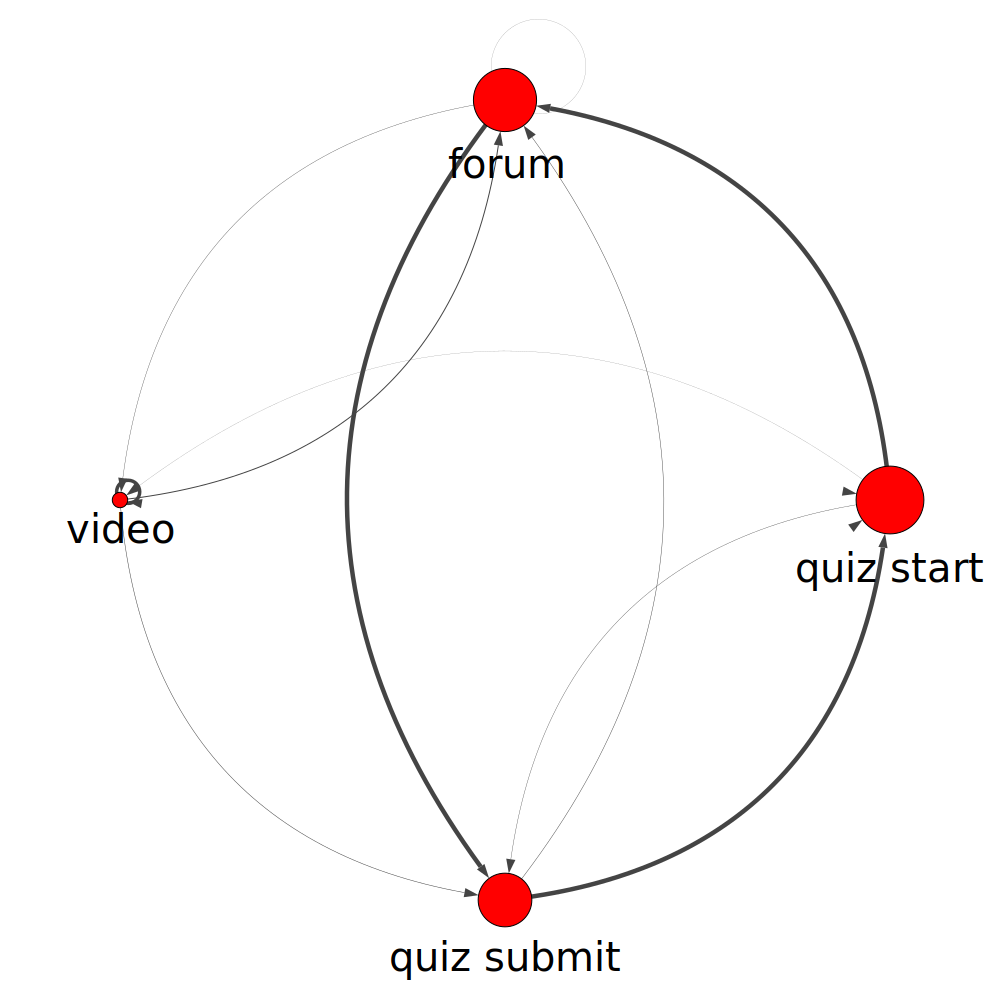
\includegraphics[width=0.7\textwidth]{../figures/example/state1.png}
\end{frame}

\begin{frame}{(Theoretical Example) Transitions Between Patterns}
  \centering
  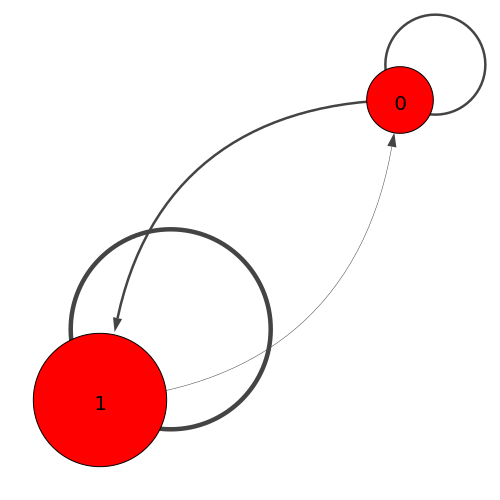
\includegraphics[width=0.7\textwidth]{../figures/example/trans.png}
\end{frame}

\begin{frame}{Why do we need a different model/representation?}
    Rule-based
    methods\footfullcite{Kizilcec:2013:LAK}\textsuperscript{,}\footfullcite{Davis:2016:EDM}
    require \textbf{knowing what you're looking for} before you look for
    it.
    \\[\baselineskip]
    We suggest instead that patterns are \textbf{latent} and may be
    difficult to specify in advance via a series of rules.
    \\[\baselineskip]
    Let the data speak: \textbf{probabilistically} discover these patterns
    from large data.
\end{frame}

\begin{frame}{Why do we need a different model/representation?}
  Previous probabilistic representations\footfullcite{Faucon:2016:EDM}
  assume that students exhibit \textbf{only one behavioral pattern over
  time}.
  \\[\baselineskip]
  We suggest that student behavior is \textbf{dynamic}, and that we should
  have a model to understand how students move between the patterns we
  discover.
  \\[\baselineskip]
  Let the data speak: \textbf{probabilistically} discover \textbf{latent
  state transition} behavior
\end{frame}

\begin{frame}{Why do we need a different model/representation?}
  Previous models \textbf{assume} a certain level of \textbf{time
  granularity}\footfullcite{Shih:2010:EDM}\textsuperscript{,}\footfullcite{Kizilcec:2013:LAK}\textsuperscript{,}\footfullcite{Faucon:2016:EDM}
  for the patterns to be discovered.
  \\[\baselineskip]
  We propose a model that is \textbf{agnostic to the time resolution
  considered} to allow it to be flexible to model different levels of
  granularity as needed.
\end{frame}

\section{Modeling Details}

\begin{frame}{The Generative Model}
  \begin{center}
    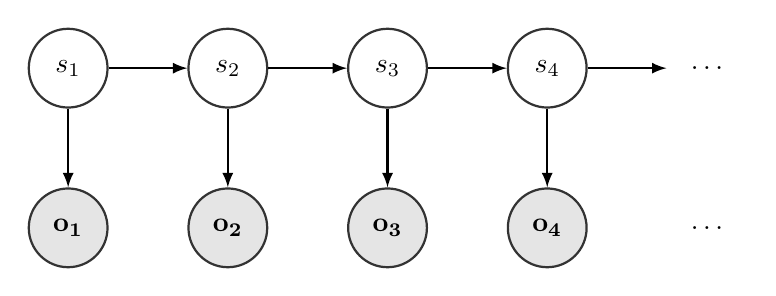
\begin{tikzpicture}
      \tikzstyle{main}=[circle, minimum size = 10mm, thick, draw =black!80, node distance = 10mm]
      \tikzstyle{observed}=[circle, minimum size = 10mm, thick, draw=black!80, node distance = 10mm, fill = black!10]
      \tikzstyle{invismain}=[circle, minimum size = 10mm, thick, draw =white!100, node distance = 10mm]
      \tikzstyle{connect}=[-latex, thick]
      \tikzstyle{box}=[rectangle, draw=black!100]

      % tags
      \node[main, fill = white!100] (s1) [] { $s_1$ };
      \node[main, fill = white!100] (s2) [right=of s1] { $s_2$ };
      \node[main, fill = white!100] (s3) [right=of s2] { $s_3$ };
      \node[main, fill = white!100] (s4) [right=of s3] { $s_4$ };
      \node[invismain, opacity=0, text opacity=1] (sn) [right=of s4] {$\ldots$};

      % words
      \node[observed] (o1) [below=of s1] { $\mathbf{o_1}$ };
      \node[observed] (o2) [below=of s2] { $\mathbf{o_2}$ };
      \node[observed] (o3) [below=of s3] { $\mathbf{o_3}$ };
      \node[observed] (o4) [below=of s4] { $\mathbf{o_4}$ };
      \node[invismain, opacity=0, text opacity=1] (on) [below=of sn] {$\ldots$};

      \path (s1) edge [connect] (s2)
        (s2) edge [connect] (s3)
        (s3) edge [connect] (s4)
        (s4) edge [connect] (sn);

      \path (s1) edge [connect] (o1);
      \path (s2) edge [connect] (o2);
      \path (s3) edge [connect] (o3);
      \path (s4) edge [connect] (o4);

    \end{tikzpicture}
  \end{center}
  \[
    \underbrace{\overbrace{\langle \overbrace{lecture}^{\text{action } a_1}
      \rightarrow\, \overbrace{quiz}^{\text{action } a_2} \rightarrow\,
      \ldots\, \rightarrow\, \overbrace{wiki}^{\text{action } a_T}
    \rangle}^{\text{observation } \mathbf{o}_1 \text{ ``generated'' from }
    s_1}, \overbrace{\langle \overbrace{wiki}^{\text{action } a_1}
      \rightarrow\, \overbrace{quiz}^{\text{action } a_2} \rightarrow\,
    \ldots \rangle}^{\text{observation } \mathbf{o}_2 \text{ ``generated'' from } s_2},
    \ldots}_{\text{student sequence } \mathbf{O}^{(\ell)}}
  \]
\end{frame}

\begin{frame}{The Generative Model}
  \begin{center}
    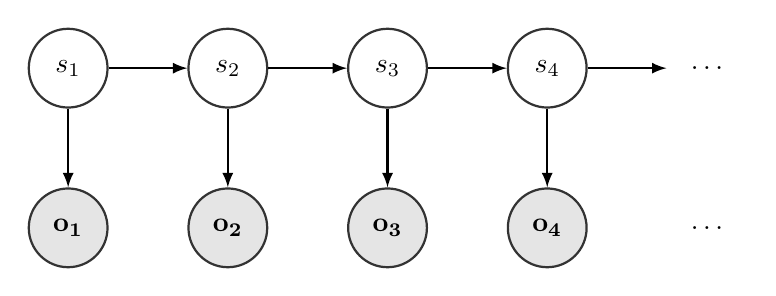
\begin{tikzpicture}
      \tikzstyle{main}=[circle, minimum size = 10mm, thick, draw =black!80, node distance = 10mm]
      \tikzstyle{observed}=[circle, minimum size = 10mm, thick, draw=black!80, node distance = 10mm, fill = black!10]
      \tikzstyle{invismain}=[circle, minimum size = 10mm, thick, draw =white!100, node distance = 10mm]
      \tikzstyle{connect}=[-latex, thick]
      \tikzstyle{box}=[rectangle, draw=black!100]

      % tags
      \node[main, fill = white!100] (s1) [] { $s_1$ };
      \node[main, fill = white!100] (s2) [right=of s1] { $s_2$ };
      \node[main, fill = white!100] (s3) [right=of s2] { $s_3$ };
      \node[main, fill = white!100] (s4) [right=of s3] { $s_4$ };
      \node[invismain, opacity=0, text opacity=1] (sn) [right=of s4] {$\ldots$};

      % words
      \node[observed] (o1) [below=of s1] { $\mathbf{o_1}$ };
      \node[observed] (o2) [below=of s2] { $\mathbf{o_2}$ };
      \node[observed] (o3) [below=of s3] { $\mathbf{o_3}$ };
      \node[observed] (o4) [below=of s4] { $\mathbf{o_4}$ };
      \node[invismain, opacity=0, text opacity=1] (on) [below=of sn] {$\ldots$};

      \path (s1) edge [connect] (s2)
        (s2) edge [connect] (s3)
        (s3) edge [connect] (s4)
        (s4) edge [connect] (sn);

      \path (s1) edge [connect] (o1);
      \path (s2) edge [connect] (o2);
      \path (s3) edge [connect] (o3);
      \path (s4) edge [connect] (o4);

    \end{tikzpicture}
  \end{center}

  Model parameters $\Lambda = (\pi, A, B)$:
  \begin{itemize}
    \item $\pi$: probability of starting student sequence in latent state
      $s_i$
    \item $A$: transition probability between latent states
    \item $B = (\lambda^{(1)}, \ldots, \lambda^{(K)})$ where
      \begin{itemize}
        \item $\lambda^{(i)} = (\pi^{(i)}, A^{(i)})$, initial probability
          and transition matrix between student \emph{actions} (e.g. view
          forum, take quiz, \ldots) for latent state $s_i$
      \end{itemize}
  \end{itemize}
\end{frame}

\begin{frame}{Inference}
    \small
    Given $\mathbf{D} = (\mathbf{O}^{(1)}, \ldots,
    \mathbf{O}^{(|\mathbf{L}|)})$, our goal is to infer the $\Lambda = (\pi, A,
    B)$ that maximizes the likelihood our model generates $\mathbf{D}$.
    \\[\baselineskip]
    Modified Baum-Welch algorithm\footfullcite{Rabiner:1990:RSR} for hidden
    Markov models. M-step updated to learn the latent state
    representations\footnote{See the full paper for more details.}:
    \begin{align*}
      \pi^{(i)}_{a} &= \frac{\sum_{\mathbf{O} \in \mathbf{D}}
      \sum_{\mathbf{o}_t \in \mathbf{O},\mathbf{o}_{t,1} = a}
      \gamma^{(\mathbf{O})}_t(i)} {\sum_{\mathbf{O} \in \mathbf{D}}
      \sum_{\mathbf{o}_t \in \mathbf{O}} \gamma^{(\mathbf{O})}_t(i)},
      \text{ and }\\
      A^{(i)}_{ab} &= \frac{\sum_{\mathbf{O} \in \mathbf{D}}
      \sum_{\mathbf{o}_t \in \mathbf{O}} \sum_{m=2,\mathbf{o}_{t,m-1}=a
      \land \mathbf{o}_{t,m} = b}^{|\mathbf{o}_{t}|}
      \gamma^{(\mathbf{O})}_t(i)} {\sum_{\mathbf{O} \in \mathbf{D}}
      \sum_{\mathbf{o}_t \in \mathbf{O}}
      \sum_{m=2,\mathbf{o}_{t,m-1}=a}^{|\mathbf{o}_{t}|}
      \gamma^{(\mathbf{O})}_t(i)}
    \end{align*}
    where $\gamma^{(\mathbf{O})}(i)$ is the posterior probability that a
    list of action sequences $\mathbf{O}$ is generated from latent state
    $i$ (efficiently recovered via Baum-Welch).
\end{frame}

\section{Experiments}

\newcommand{\textretrieval}{textretrieval-001}
\newcommand{\sustain}{sustain-001}
\newcommand{\UIUC}{UIUC}

\begin{frame}{Data}
\begin{table}
  \begin{center}
    \caption{Statistics about the sequences extracted from the two MOOCs.}
    \label{table:datasets}
    \begin{tabular}{rrrr}
      \textbf{MOOC} & \textbf{Students} & \textbf{Sequences} & \textbf{Avg.
      $|\mathbf{s}|$}\\\hline
      \textretrieval{} & 18,941 & 85,240 & 7.31\\
      \sustain{} & 85,240 & 231,881 & 15.4
    \end{tabular}
  \end{center}
\end{table}
\end{frame}

\begin{frame}{Behavior Pattern 0 ($K = 4$)}
  \centering
  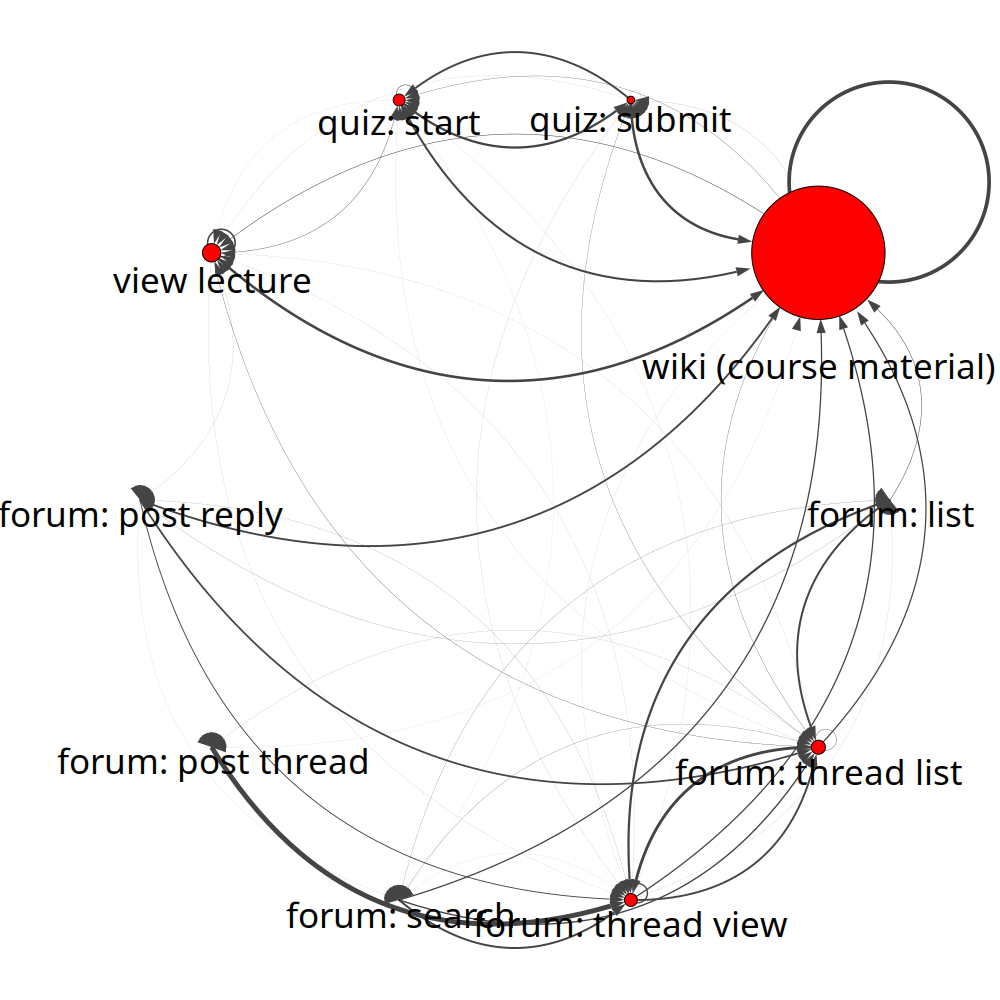
\includegraphics[width=0.70\textwidth]{../figures/text-4state/state0.png}
\end{frame}

\begin{frame}{Behavior Pattern 1 ($K = 4$)}
  \centering
  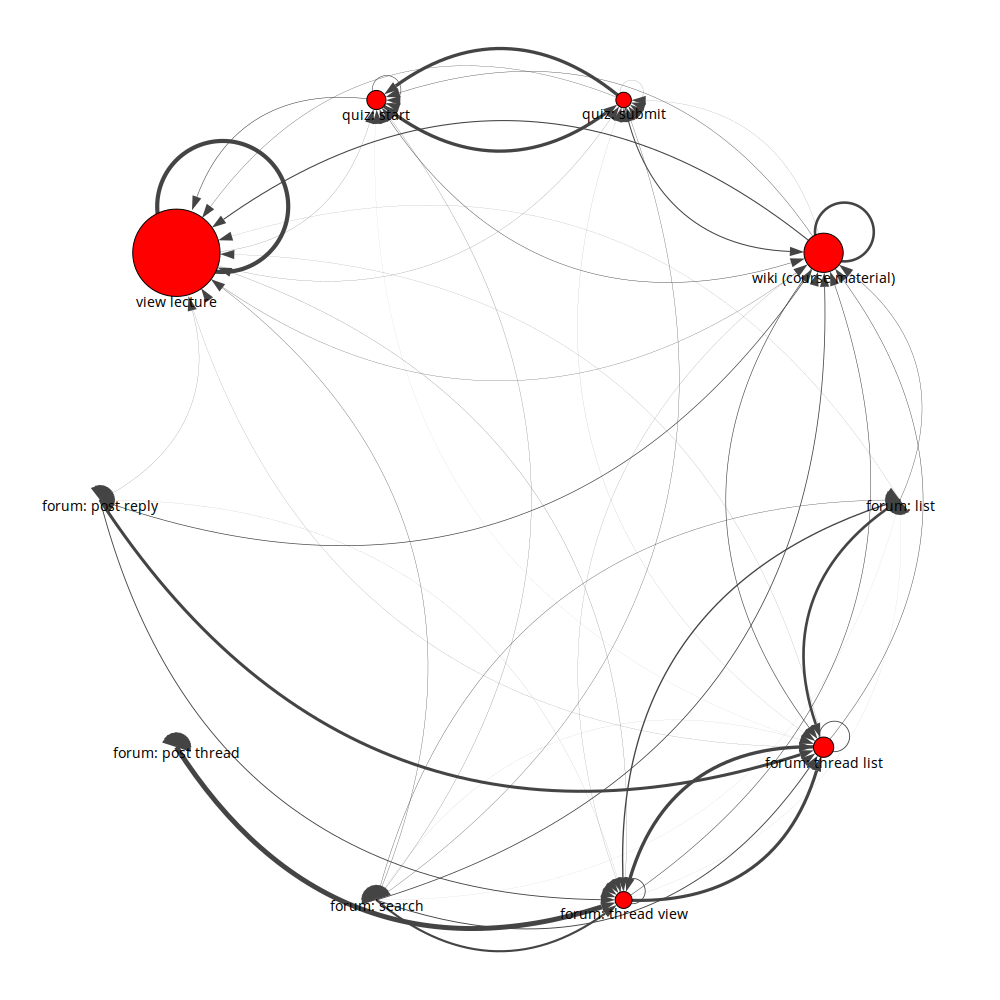
\includegraphics[width=0.70\textwidth]{../figures/text-4state/state1.png}
\end{frame}

\begin{frame}{Behavior Pattern 2 ($K = 4$)}
  \centering
  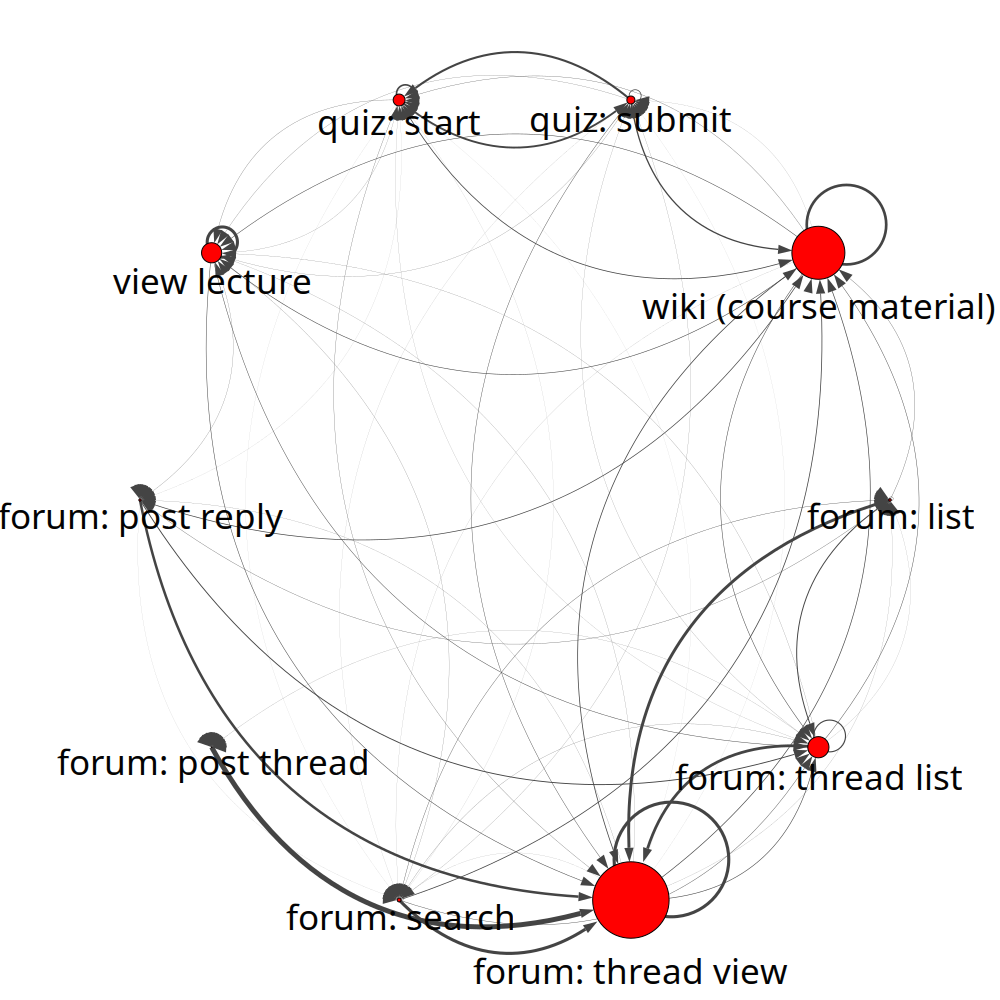
\includegraphics[width=0.70\textwidth]{../figures/text-4state/state2.png}
\end{frame}

\begin{frame}{Behavior Pattern 3 ($K = 4$)}
  \centering
  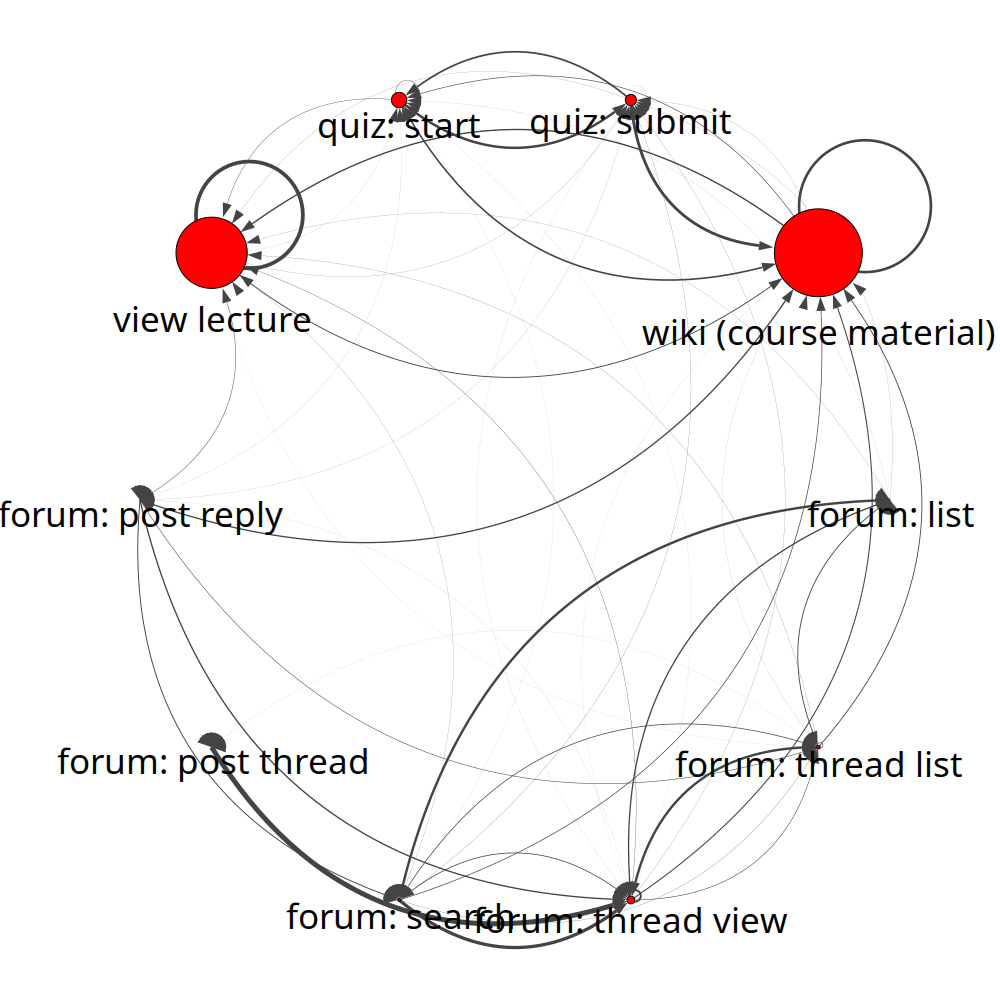
\includegraphics[width=0.70\textwidth]{../figures/text-4state/state3.png}
\end{frame}

\begin{frame}{A Closer Look}
 State 1 and state 3 capture most of the quiz taking behavior, but are
 actually quite different from each other. Let's look closer\ldots
\end{frame}

\begin{frame}{``For more on this, it's time for \emph{A Closer Look}.''
    (State 1)}
  \centering
  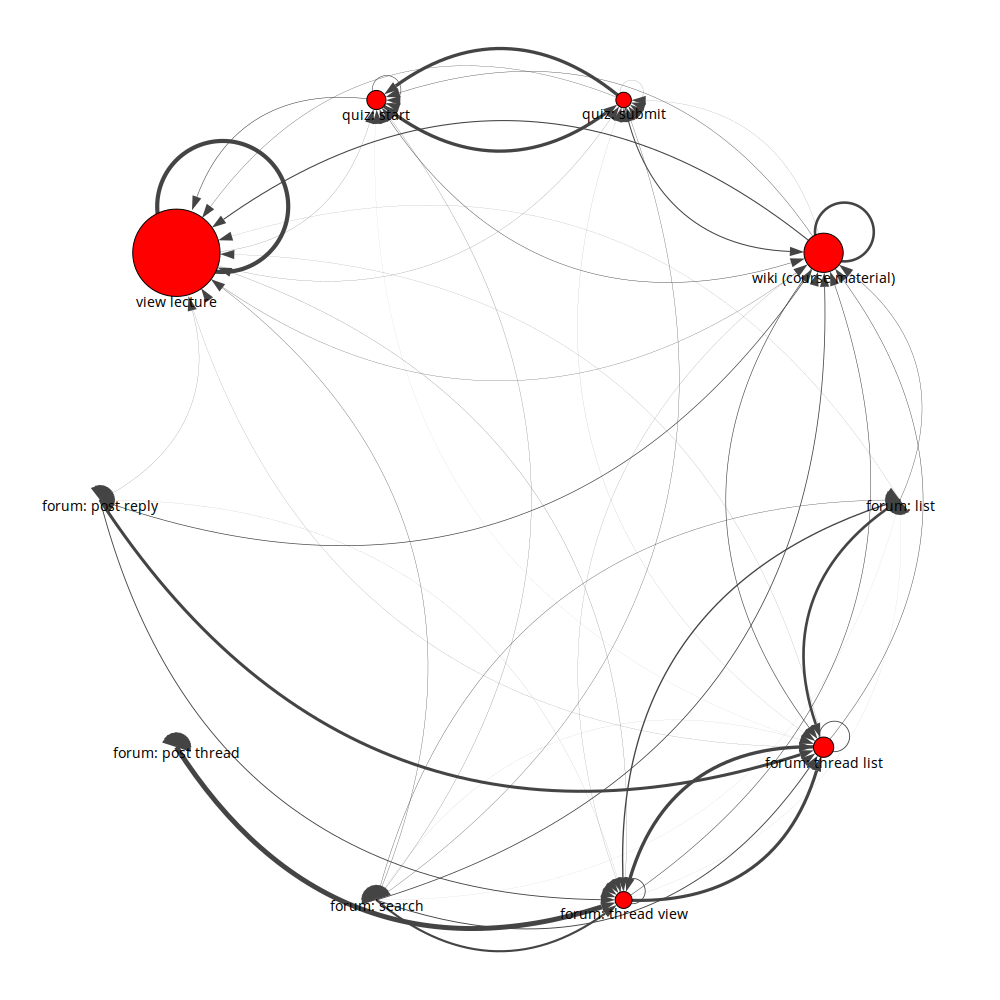
\includegraphics[width=0.70\textwidth]{../figures/text-4state/state1.png}
\end{frame}

\begin{frame}{``For more on this, it's time for \emph{A Closer Look}.''
    (State 3)}
  \centering
  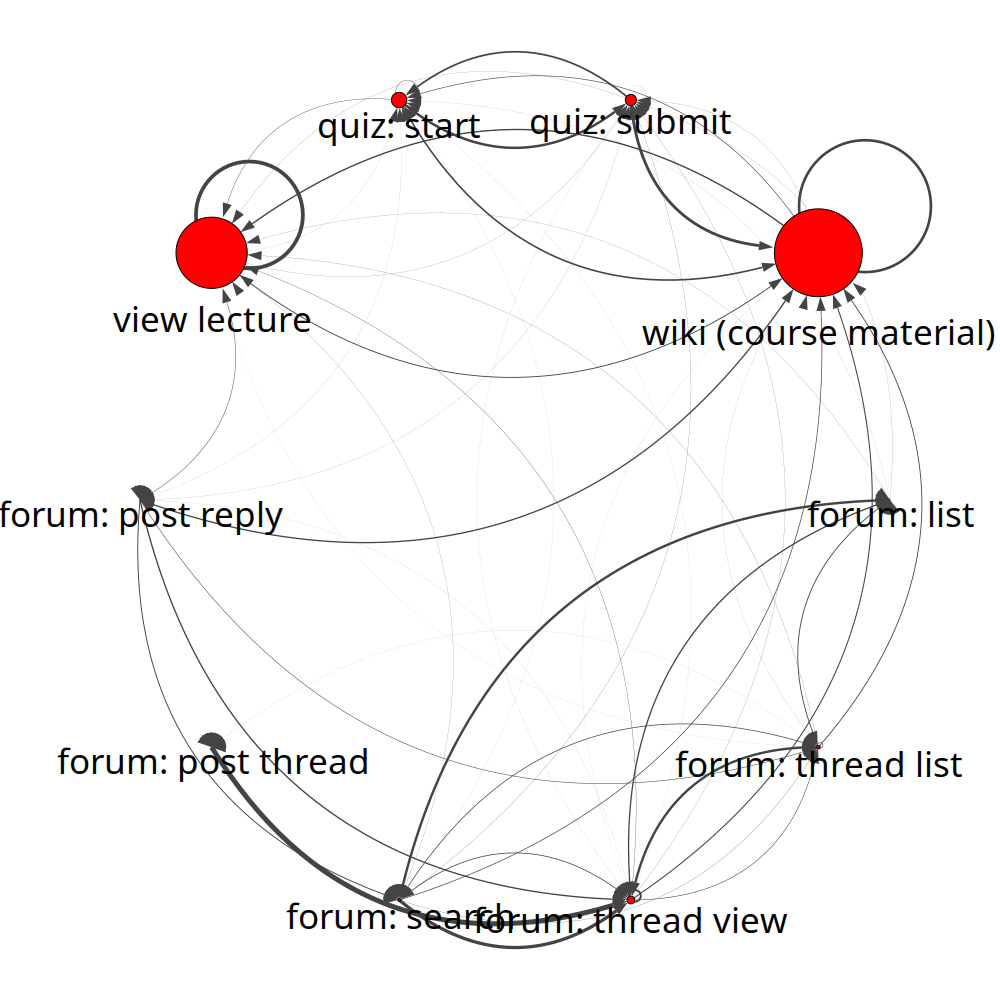
\includegraphics[width=0.70\textwidth]{../figures/text-4state/state3.png}
\end{frame}

\begin{frame}{A Look at Transitions (All)}
  \centering
  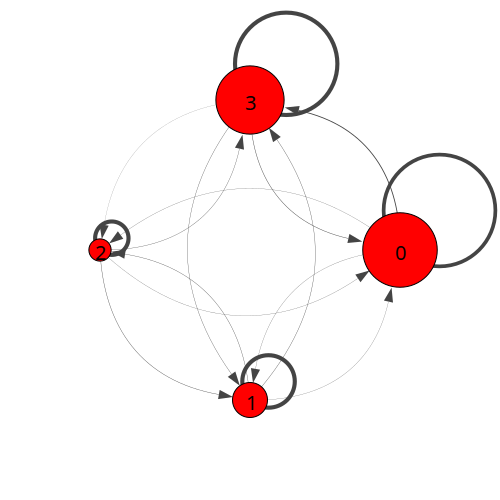
\includegraphics[width=0.70\textwidth]{../figures/trans-comp/trans-avg.png}
\end{frame}

\begin{frame}{A Look at Transitions (Perfect retrofit)}
  \centering
  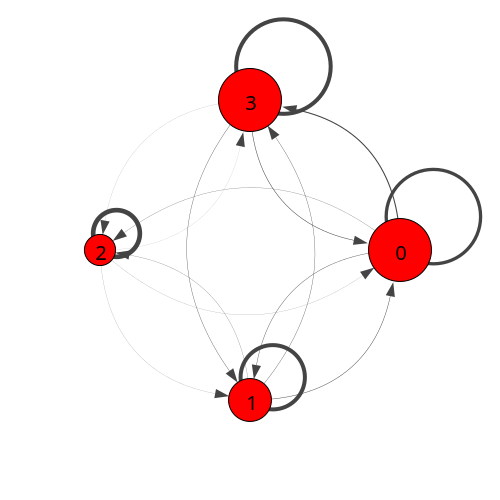
\includegraphics[width=0.70\textwidth]{../figures/trans-comp/trans-perfect.png}
\end{frame}

\begin{frame}{A Look at Transitions (Low retrofit)}
  \centering
  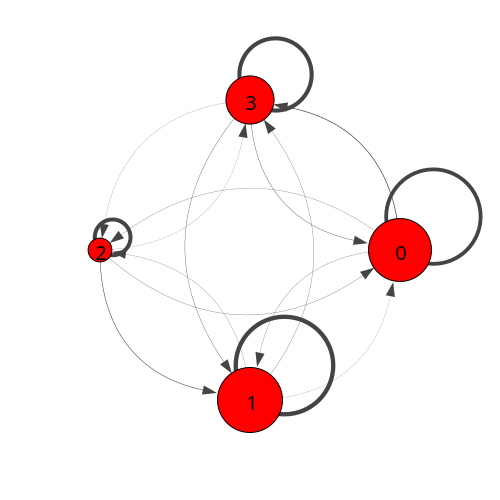
\includegraphics[width=0.70\textwidth]{../figures/trans-comp/trans-low.png}
\end{frame}

\begin{frame}{A Look at Transitions (All)}
  \centering
  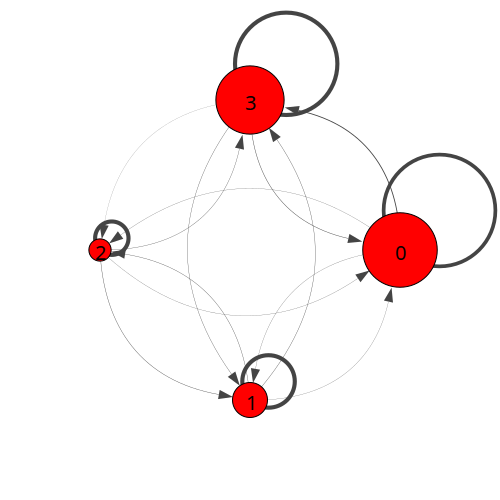
\includegraphics[width=0.70\textwidth]{../figures/trans-comp/trans-avg.png}
\end{frame}

\begin{frame}{Ranking experiment}
\begin{table}
  \centering
  \caption{Average rank for ``perfect'' and ``low'' student groups in the
  ranked lists associated with the four latent states found by a 2L-HMM.
  $\dagger$ indicates statistically significant different mean ranks at $p
  < 0.01$ according to an unpaired $t$-test.}
  \label{table:mean-rank}
  \begin{tabular}{r|rrrrr}
    \textbf{Group} & \textbf{State 0} & \textbf{State
  1}\textsuperscript\textdagger &
    \textbf{State 2}\textsuperscript\textdagger & \textbf{State 3} & \textbf{State 2
    $\rightarrow$ 2}\textsuperscript\textdagger\\\hline
    \textbf{Perfect} & 975.3  & 1001.5 & 999.0  & 1056.5 & 939.6\\
    \textbf{Low}     & 1024.9 & 816.4  & 1230.5 & 1161.2 & 1187.4\\
  \end{tabular}
\end{table}
\end{frame}

\section{Concluding Remarks}

\begin{frame}{Conclusion}
\small
We proposed using \textbf{\alert{Two-layer Hidden Markov Models}} to
discover \textbf{latent student behavior patterns} as well as the
\textbf{transitioning behavior between them}. The patterns we extract are
meaningful and can be used to extract features that correlate with student
performance.
\\[\baselineskip]
The code for learning the parameters of a 2L-HMM is available as part of
the \textsc{MeTA} toolkit\footfullcite{Massung:2016:ACL} available at
\url{https://meta-toolkit.org}.
\\[\baselineskip]
The code for generating the visualizations for a 2L-HMM on MOOC data is
available on GitHub: \url{https://github.com/skystrife/clickstream-hmm}
\end{frame}

\begin{frame}
    \centering
    \Huge
    Thank you!
\end{frame}

\end{document}
